\documentclass[tikz,border=2mm]{standalone}
\usetikzlibrary{shapes.misc}
\begin{document}
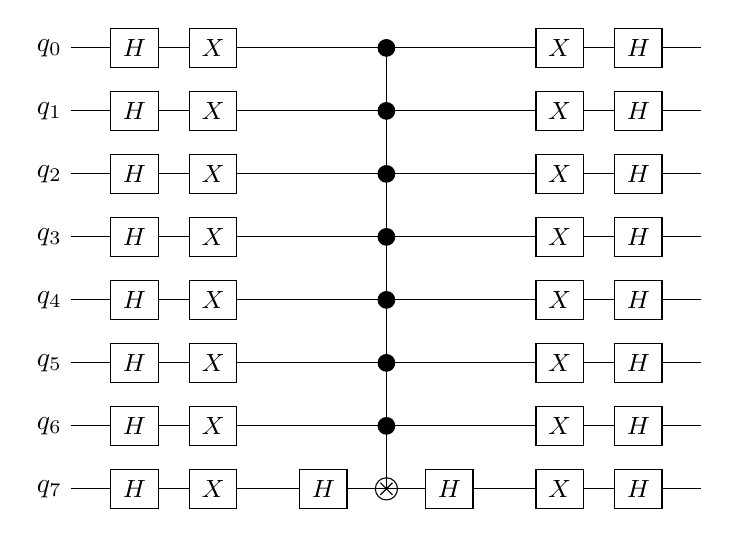
\begin{tikzpicture}
\foreach \i in {0,1,2,3,4,5,6,7} {
    \draw (0,-\i*0.8) -- (8,-\i*0.8);
    \node[anchor=east] at (0,-\i*0.8) {$q_\i$};
    \draw[fill=white] (0.5,-\i*0.8-0.25) rectangle (1.1,-\i*0.8+0.25) node[pos=0.5, font=\small] {$H$};
    \draw[fill=white] (1.5,-\i*0.8-0.25) rectangle (2.1,-\i*0.8+0.25) node[pos=0.5, font=\small] {$X$};
    
    \draw[fill=white] (5.9,-\i*0.8-0.25) rectangle (6.5,-\i*0.8+0.25) node[pos=0.5, font=\small] {$X$};
    \draw[fill=white] (6.9,-\i*0.8-0.25) rectangle (7.5,-\i*0.8+0.25) node[pos=0.5, font=\small] {$H$};
}
\draw[fill=white] (2.9,-7*0.8-0.25) rectangle (3.5,-7*0.8+0.25) node[pos=0.5, font=\small] {$H$};
\draw[fill=white] (4.5,-7*0.8-0.25) rectangle (5.1,-7*0.8+0.25) node[pos=0.5, font=\small] {$H$};

\draw (4,0) -- (4,-7*0.8);
\foreach \i in {0,1,2,3,4,5,6} {
    \filldraw (4,-\i*0.8) circle (3pt);
}
\draw (4,-7*0.8) circle (4pt) node[cross out, draw, inner sep=2pt] {};
\end{tikzpicture}
\end{document}
